%
% offen.tex
%
% (c) 2024 Prof Dr Andreas Müller
%
\begin{figure}
\centering
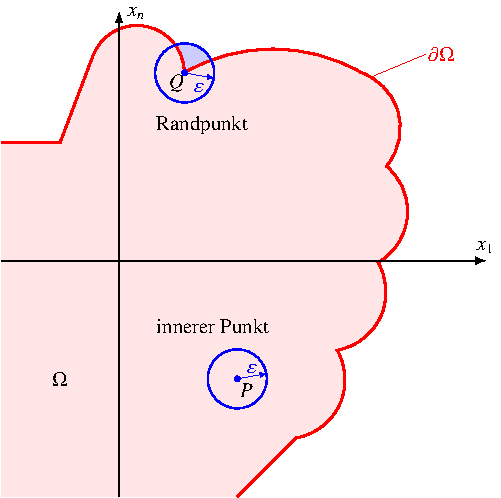
\includegraphics{chapters/040-felder/images/offen.pdf}
\caption{Jeder Punkt einer offenen Menge $\Omega$ besitzt eine kleine
Umgebung, die ebenfalls in der Menge enthalten ist.
Punkte, deren Umgebungen immer Punkte von $\Omega$ und Punkte des
Komplementes $\mathbb{R}^n\setminus\Omega$ enhalten, liegen auf dem
Rand $\partial\Omega$ von $\Omega$.
\label{buch:felder:fundamentallemma:fig:offen}}
\end{figure}
